\ifx\allfiles\undefined
\documentclass[12pt, a4paper, oneside, UTF8]{ctexbook}
\def\path{../config}
\usepackage{amsmath}
\usepackage{amsthm}
\usepackage{array}
\usepackage{amssymb}
\usepackage{graphicx}
\usepackage{mathrsfs}
\usepackage{enumitem}
\usepackage{geometry}
\usepackage[colorlinks, linkcolor=black]{hyperref}
\usepackage{stackengine}
\usepackage{yhmath}
\usepackage{extarrows}
% \usepackage{unicode-math}
\usepackage{esint}
\usepackage{multirow}
\usepackage{fancyhdr}
\usepackage[dvipsnames, svgnames]{xcolor}
\usepackage{listings}
\usepackage{float} % Required for the H float option
\definecolor{mygreen}{rgb}{0,0.6,0}
\definecolor{mygray}{rgb}{0.5,0.5,0.5}
\definecolor{mymauve}{rgb}{0.58,0,0.82}
\definecolor{NavyBlue}{RGB}{0,0,128}
\definecolor{Rhodamine}{RGB}{255,0,255}
\definecolor{PineGreen}{RGB}{0,128,0}

\graphicspath{ {figures/},{../figures/}, {config/}, {../config/} }

\linespread{1.6}

\geometry{
    top=25.4mm, 
    bottom=25.4mm, 
    left=20mm, 
    right=20mm, 
    headheight=2.17cm, 
    headsep=4mm, 
    footskip=12mm
}

\setenumerate[1]{itemsep=5pt,partopsep=0pt,parsep=\parskip,topsep=5pt}
\setitemize[1]{itemsep=5pt,partopsep=0pt,parsep=\parskip,topsep=5pt}
\setdescription{itemsep=5pt,partopsep=0pt,parsep=\parskip,topsep=5pt}

\lstset{
    language=Mathematica,
    basicstyle=\tt,
    breaklines=true,
    keywordstyle=\bfseries\color{NavyBlue}, 
    emphstyle=\bfseries\color{Rhodamine},
    commentstyle=\itshape\color{black!50!white}, 
    stringstyle=\bfseries\color{PineGreen!90!black},
    columns=flexible,
    numbers=left,
    numberstyle=\footnotesize,
    frame=tb,
    breakatwhitespace=false,
} 

\lstset{
    language=TeX, % 设置语言为 TeX
    basicstyle=\ttfamily, % 使用等宽字体
    breaklines=true, % 自动换行
    keywordstyle=\bfseries\color{NavyBlue}, % 关键字样式
    emphstyle=\bfseries\color{Rhodamine}, % 强调样式
    commentstyle=\itshape\color{black!50!white}, % 注释样式
    stringstyle=\bfseries\color{PineGreen!90!black}, % 字符串样式
    columns=flexible, % 列的灵活性
    numbers=left, % 行号在左侧
    numberstyle=\footnotesize, % 行号字体大小
    frame=tb, % 顶部和底部边框
    breakatwhitespace=false % 不在空白处断行
}

% \begin{lstlisting}[language=TeX] ... \end{lstlisting}

% 定理环境设置
\usepackage[strict]{changepage} 
\usepackage{framed}

\definecolor{greenshade}{rgb}{0.90,1,0.92}
\definecolor{redshade}{rgb}{1.00,0.88,0.88}
\definecolor{brownshade}{rgb}{0.99,0.95,0.9}
\definecolor{lilacshade}{rgb}{0.95,0.93,0.98}
\definecolor{orangeshade}{rgb}{1.00,0.88,0.82}
\definecolor{lightblueshade}{rgb}{0.8,0.92,1}
\definecolor{purple}{rgb}{0.81,0.85,1}

\theoremstyle{definition}
\newtheorem{myDefn}{\indent Definition}[section]
\newtheorem{myLemma}{\indent Lemma}[section]
\newtheorem{myThm}[myLemma]{\indent Theorem}
\newtheorem{myCorollary}[myLemma]{\indent Corollary}
\newtheorem{myCriterion}[myLemma]{\indent Criterion}
\newtheorem*{myRemark}{\indent Remark}
\newtheorem{myProposition}{\indent Proposition}[section]

\newenvironment{formal}[2][]{%
	\def\FrameCommand{%
		\hspace{1pt}%
		{\color{#1}\vrule width 2pt}%
		{\color{#2}\vrule width 4pt}%
		\colorbox{#2}%
	}%
	\MakeFramed{\advance\hsize-\width\FrameRestore}%
	\noindent\hspace{-4.55pt}%
	\begin{adjustwidth}{}{7pt}\vspace{2pt}\vspace{2pt}}{%
		\vspace{2pt}\end{adjustwidth}\endMakeFramed%
}

\newenvironment{definition}{\vspace{-\baselineskip * 2 / 3}%
	\begin{formal}[Green]{greenshade}\vspace{-\baselineskip * 4 / 5}\begin{myDefn}}
	{\end{myDefn}\end{formal}\vspace{-\baselineskip * 2 / 3}}

\newenvironment{theorem}{\vspace{-\baselineskip * 2 / 3}%
	\begin{formal}[LightSkyBlue]{lightblueshade}\vspace{-\baselineskip * 4 / 5}\begin{myThm}}%
	{\end{myThm}\end{formal}\vspace{-\baselineskip * 2 / 3}}

\newenvironment{lemma}{\vspace{-\baselineskip * 2 / 3}%
	\begin{formal}[Plum]{lilacshade}\vspace{-\baselineskip * 4 / 5}\begin{myLemma}}%
	{\end{myLemma}\end{formal}\vspace{-\baselineskip * 2 / 3}}

\newenvironment{corollary}{\vspace{-\baselineskip * 2 / 3}%
	\begin{formal}[BurlyWood]{brownshade}\vspace{-\baselineskip * 4 / 5}\begin{myCorollary}}%
	{\end{myCorollary}\end{formal}\vspace{-\baselineskip * 2 / 3}}

\newenvironment{criterion}{\vspace{-\baselineskip * 2 / 3}%
	\begin{formal}[DarkOrange]{orangeshade}\vspace{-\baselineskip * 4 / 5}\begin{myCriterion}}%
	{\end{myCriterion}\end{formal}\vspace{-\baselineskip * 2 / 3}}
	

\newenvironment{remark}{\vspace{-\baselineskip * 2 / 3}%
	\begin{formal}[LightCoral]{redshade}\vspace{-\baselineskip * 4 / 5}\begin{myRemark}}%
	{\end{myRemark}\end{formal}\vspace{-\baselineskip * 2 / 3}}

\newenvironment{proposition}{\vspace{-\baselineskip * 2 / 3}%
	\begin{formal}[RoyalPurple]{purple}\vspace{-\baselineskip * 4 / 5}\begin{myProposition}}%
	{\end{myProposition}\end{formal}\vspace{-\baselineskip * 2 / 3}}


\newtheorem{example}{\indent \color{SeaGreen}{Example}}[section]
\renewcommand{\proofname}{\indent\textbf{\textcolor{TealBlue}{Proof}}}
\newenvironment{solution}{\begin{proof}[\indent\textbf{\textcolor{TealBlue}{Solution}}]}{\end{proof}}

% 自定义命令的文件

\def\d{\mathrm{d}}
\def\R{\mathbb{R}}
%\newcommand{\bs}[1]{\boldsymbol{#1}}
%\newcommand{\ora}[1]{\overrightarrow{#1}}
\newcommand{\myspace}[1]{\par\vspace{#1\baselineskip}}
\newcommand{\xrowht}[2][0]{\addstackgap[.5\dimexpr#2\relax]{\vphantom{#1}}}
\newenvironment{mycases}[1][1]{\linespread{#1} \selectfont \begin{cases}}{\end{cases}}
\newenvironment{myvmatrix}[1][1]{\linespread{#1} \selectfont \begin{vmatrix}}{\end{vmatrix}}
\newcommand{\tabincell}[2]{\begin{tabular}{@{}#1@{}}#2\end{tabular}}
\newcommand{\pll}{\kern 0.56em/\kern -0.8em /\kern 0.56em}
\newcommand{\dive}[1][F]{\mathrm{div}\;\boldsymbol{#1}}
\newcommand{\rotn}[1][A]{\mathrm{rot}\;\boldsymbol{#1}}

% 修改参数改变封面样式,0 默认原始封面、内置其他1、2、3种封面样式
\def\myIndex{0}


\ifnum\myIndex>0
    \input{\path/cover_package_\myIndex}
\fi

\def\myTitle{标题:一份LaTeX笔记模板}
\def\myAuthor{作者名称}
\def\myDateCover{封面日期: \today}
\def\myDateForeword{前言页显示日期: \today}
\def\myForeword{前言标题}
\def\myForewordText{
    
    这是一个基于\LaTeX{}的模板,用于撰写学习笔记。

    模板旨在提供一个简单、易用的框架,以便你能够专注于内容,而不是排版细节,如不是专业者,不建议使用者在模板细节上花费太多时间,而是直接使用模板进行笔记撰写。遇到问题,再进行调整解决。
}
\def\mySubheading{副标题}


\begin{document}
\input{\path/cover_text_\myIndex.tex}

\newpage
\thispagestyle{empty}
\begin{center}
    \Huge\textbf{\myForeword}
\end{center}
\myForewordText
\begin{flushright}
    \begin{tabular}{c}
        \myDateForeword
    \end{tabular}
\end{flushright}

\newpage
\pagestyle{plain}
\setcounter{page}{1}
\pagenumbering{Roman}
\tableofcontents

\newpage
\pagenumbering{arabic}
\setcounter{chapter}{-1}
\setcounter{page}{1}

\pagestyle{fancy}
\fancyfoot[C]{\thepage}
\renewcommand{\headrulewidth}{0.4pt}
\renewcommand{\footrulewidth}{0pt}








\else
\fi

\chapter{配合比计算}

\section{配合比计算的基本原理}
配合比计算是土木工程中非常重要的一环,主要用于确定混凝土或砂浆等材料的组成比例,以满足工程设计要求。配合比计算的基本原理包括以下几个方面:
\begin{itemize}
	\item \textbf{和易性要求(和易性包括流动性、粘聚性和保水性)}
	\item \textbf{强度等级要求}
	\item \textbf{耐久性要求}
	\item \textbf{经济原则}
\end{itemize}

\begin{corollary}
	{
		{\color{red}强度等级要求和耐久性指标}是给水胶比($\frac{W}{B}$)设置了一个最大值限制,因为加水可以提高流动性,但是会降低强度和耐久性

		和易性要求(或者更直接一点是和易性中流动性)是给单位用水量设置了一个最小值限制,因为水泥浆的流动性和粘聚性与单位用水量密切相关。
		
		细骨料和粗骨料也会影响流动性和粘聚性,{\color{red}在满足粘聚性和保水性基础上,尽量选择较小的砂率。}
		}
\end{corollary}

\begin{table}[H]
	\centering
	\renewcommand{\arraystretch}{1.5}
	\setlength{\tabcolsep}{30pt}
	\begin{tabular}{|c|c|c|}
		\hline
		参数名称 & 含义 & 备注 \\
		\hline
		$f_{cu,k}$ & 混凝土强度的工厂生产参考值 &  \\
		\hline
		$f_{ce,k}$ & 水泥强度等级标准值 &  \\
		\hline
		$f_{ce}$ & 28天标准养护下的胶砂抗压强度 &  $f_{ce} = \gamma_f \gamma_s \gamma_{cfce,k}$\\
		\hline
		$\gamma_f$ & 与粉煤灰相关的富余系数 &	一般不用  \\
		\hline
		$\gamma_s$ & 与矿渣掺合物相关的富余系数 & 一般不用 \\
		\hline
		$\gamma_c$ & 与等级相关的强度富余系数 &  \\
		\hline
		$f_{cu,0}$ & 混凝土强度的保证数 & $f_{cu,0} = f_{cu,k}+ 1.645 \sigma$ \\
		\hline
		$W$ & 用水量 &  \\
		\hline
		$B$ & 胶凝材料用量 &  \\
		\hline
		$S$ & 细骨料 &  \\
		\hline
		$G$ & 粗骨料 &  \\
		\hline
	\end{tabular}
	\caption{参数说明}
\end{table}

\begin{remark}
	\[ f_{cu,0} = \left\{ \begin{array}{ll}
f_{cu,k} + 1.645\sigma & (f_{cu,k} < C60) \\
1.15f_{cu,k} & (f_{cu,k} \geq C60)
\end{array} \right. \]
鲍罗米公式:
$$\frac{W}{B} = \frac{\alpha_a f_{ce}}{f_{cu,0} + \alpha_a \alpha_b f_{ce}}$$
$$\text{砂率}=\frac{m_S}{m_S + m_G}$$

$\alpha_a$、$\alpha_b$ —— 与粗骨料有关的回归系数,可通过历史资料统计得到,若无统计资料,可采用《普通混凝土配合比设计规程》(JGJ 55—2011)提供的经验值:采用碎石时 $\alpha_a = 0.53$,$\alpha_b = 0.20$;采用卵石时 $\alpha_a = 0.49$,$\alpha_b = 0.13$
\end{remark}

\begin{table}[H]
	\centering
	\renewcommand{\arraystretch}{1.5}
	\setlength{\tabcolsep}{30pt}
	\begin{tabular}{|c|c|c|}
		\hline
		下标参数名称 & 含义 & 备注 \\
		\hline
		$ce$ & cementitious materials & 是指胶凝材料 \\
		\hline
		$k$ & characteristic value &  特征值,等级值\\
		\hline
		$cu$ & cube  &	混凝土立方体 \\
		\hline
	\end{tabular}
	\caption{下标参数说明}
\end{table}

\subsection{一些参数说明}

\begin{figure}[H]
	\centering
	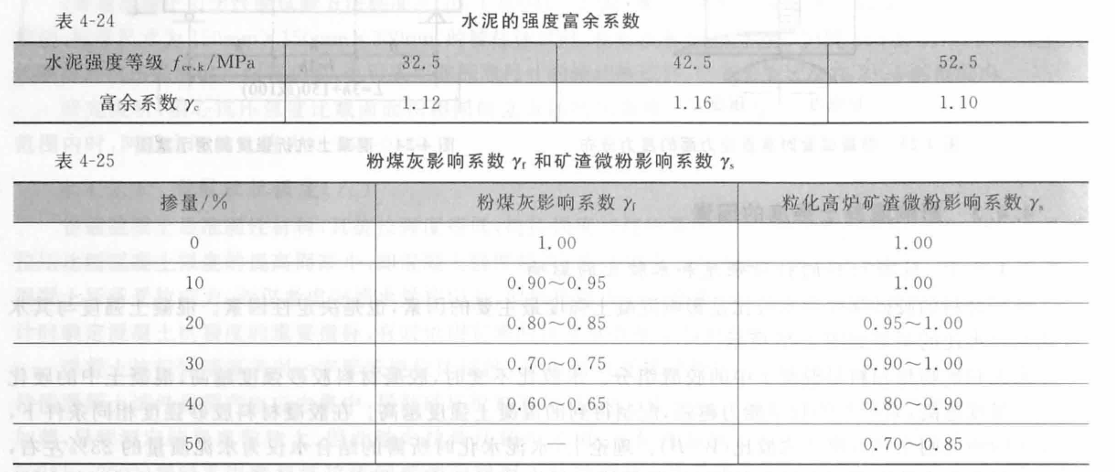
\includegraphics[width=0.8\textwidth]{../figure/5.png}
	\caption{强度富余系数的查表}
	\label{fig:strength_coefficient}
\end{figure}

\begin{figure}[H]
	\centering
	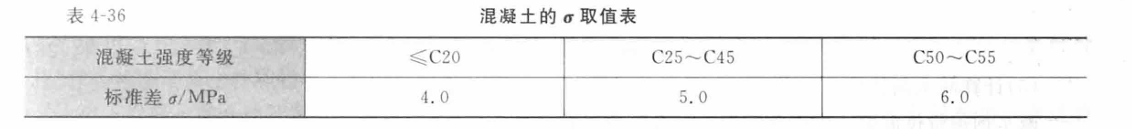
\includegraphics[width=0.8\textwidth]{../figure/2.png}
	\caption{标准差参数}
	\label{fig:standard_deviation}
\end{figure}



\section{体积法与查表细节}
\[
\begin{array}{c}
\frac{m_{co}}{p_c} + \frac{m_{go}}{p_g} + \frac{m_{so}}{p_s} + \frac{m_{wo}}{p_w} + 0.01\alpha = 1 \\
\text{砂率} = \frac{m_{s}}{m_{s} + m_{go}} \times 100\% 
\end{array}
\]

正如下表的伪代码所给出的计算流程一样,我们在计算中需要根据上文提到几个计算要求(强度、耐久性、和易性)来进行检验,以便满足要求。

以下有先后顺序:
\begin{enumerate}
	\item 根据环境对水胶比检验
	\item 根据粒径对砂率的检验
	\item 根据粒径和坍落度对最大用水量的检验
	\item 根据水胶比对胶凝材料最小用量检验
\end{enumerate}

\begin{figure}[H]
	\centering
	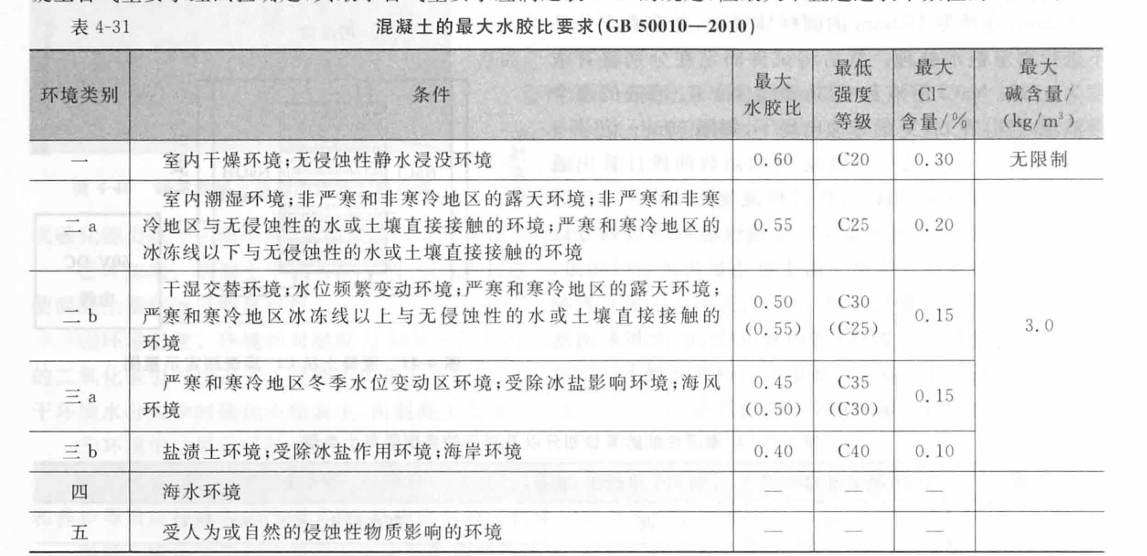
\includegraphics[width=0.8\textwidth]{../figure/1.png}
	\caption{水胶比检验}
	\label{fig:water_cement_ratio}
\end{figure}

\begin{figure}[H]
	\centering
	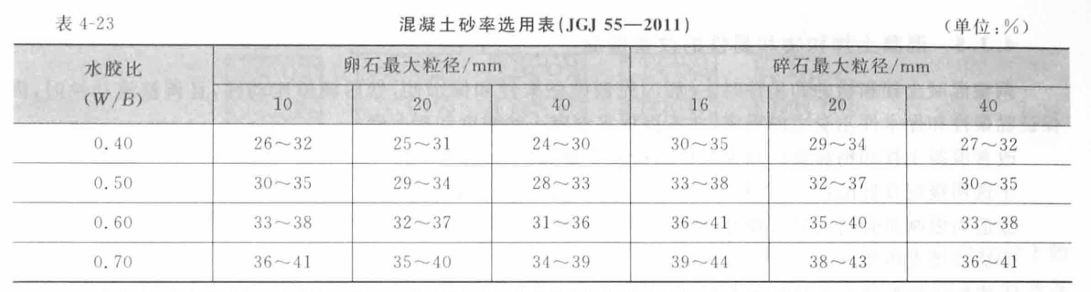
\includegraphics[width=0.8\textwidth]{../figure/8.png}
	\caption{砂率的检验}
	\label{fig:sand_rate_check}
\end{figure}

\begin{figure}[H]
	\centering
	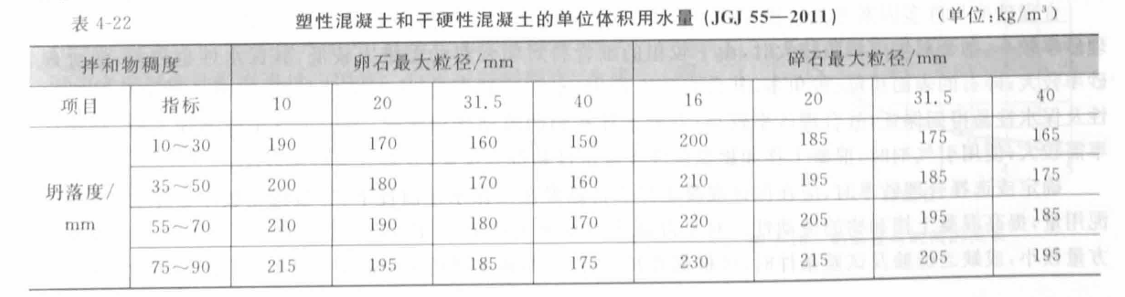
\includegraphics[width=0.8\textwidth]{../figure/6.png}
	\caption{最大用水量的查表(上)}
	\label{fig:min_water_check}
\end{figure}

\begin{figure}[H]
	\centering
	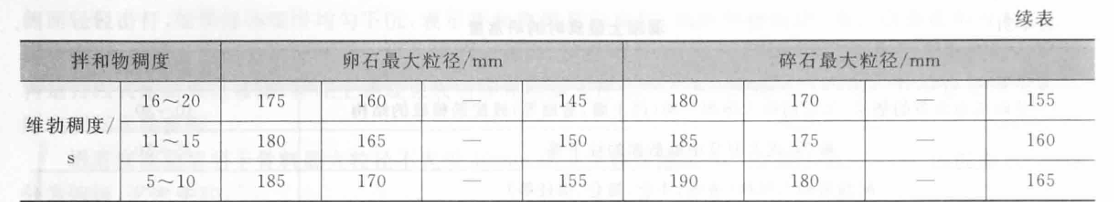
\includegraphics[width=0.8\textwidth]{../figure/7.png}
	\caption{最大用水量的查表(下)}
	\label{fig:min_water_check_lower}
\end{figure}

\begin{remark}
	注意:这里坍落度大于90,还得增加用水量,比如说200-90=110$kg/m^3$,此时需要增加$5\times \frac{110}{20}=27.5kg/m^3$
\end{remark}

\begin{figure}[H]
	\centering
	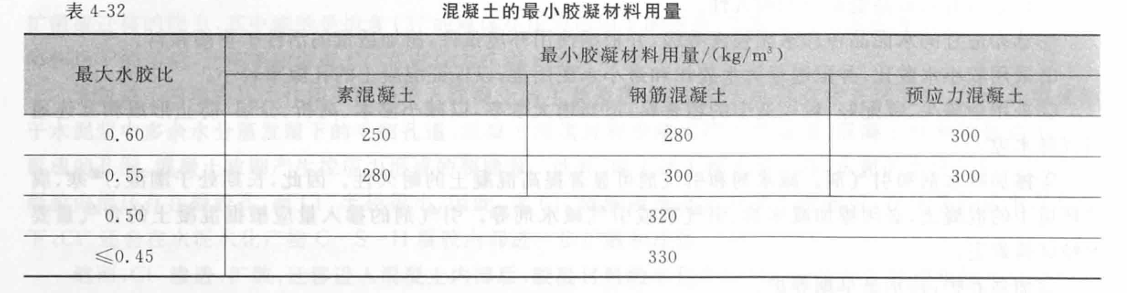
\includegraphics[width=0.8\textwidth]{../figure/3.png}
	\caption{最大用水量的说明}
	\label{fig:min_water_explanation}
\end{figure}

\begin{figure}[H]
	\centering
	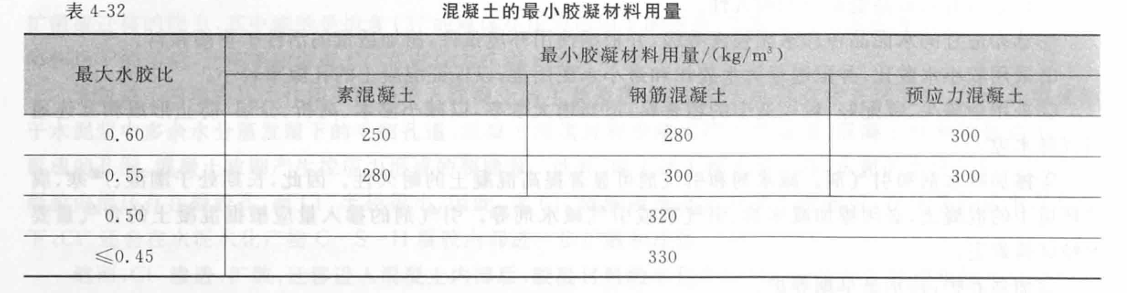
\includegraphics[width=0.8\textwidth]{../figure/3.png}
	\caption{胶凝材料用量的检验(上)}
	\label{fig:cementitious_material_check_upper}
\end{figure}

\begin{figure}[H]
	\centering
	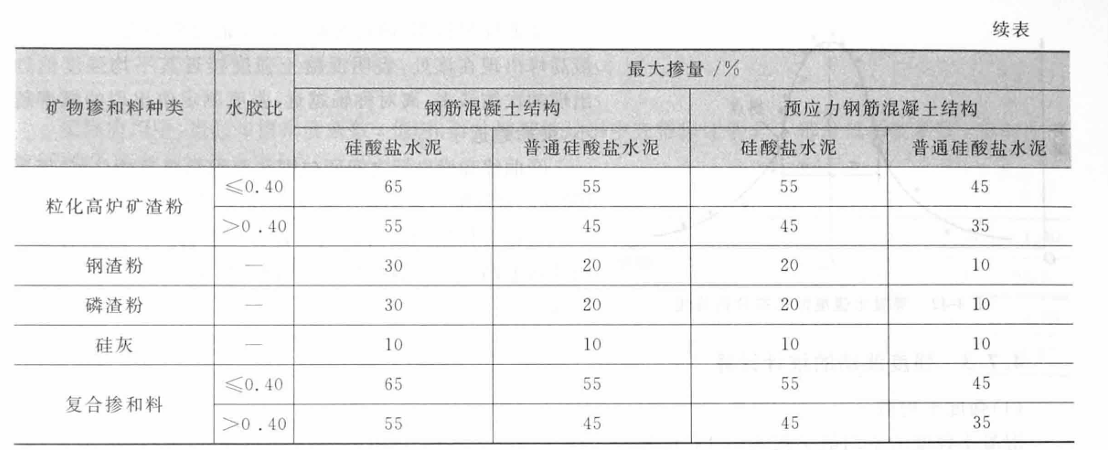
\includegraphics[width=0.8\textwidth]{../figure/4.png}
	\caption{胶凝材料用量的检验(下)}
	\label{fig:cementitious_material_check_lower}
\end{figure}


\begin{algorithm}[H]
\caption{混凝土配合比计算流程伪代码}
\begin{algorithmic}[1]

\State \textbf{输入:} $f_{ce,k}$, $f_{cu,k}$

\State $f_{ce} \gets \gamma_f \gamma_s \gamma_c f_{ce,k}$

\State $f_{cu,0} \gets f_{cu,k} + 1.645\sigma$ \Comment{95\%置信度,由经验公式}

\State 根据经验公式:
\[
\frac{W}{B} = \frac{\alpha_a f_{ce}}{f_{cu,0} + \alpha_a \alpha_b f_{ce}}
\]

\State 查表,根据环境确定水胶比,取小值为水胶比(需要考虑强度等级和耐久性条件)

\State 计算水胶比 $W/B$

\If{掺杂减水剂}
	\State $m_{w0}=m_{wL} \times (1 - \beta)$,$\beta$为减水率,$m_{wL}$为掺杂减水剂前的用水量
\EndIf

\If{给出W}
	\State 计算胶凝材料用量 $B$:$B = \frac{W}{W/B}$
	\State 根据粒径查出砂率
	\State 检查胶凝材料使用量是否满足耐久性条件,取最大值为胶凝材料用量
	\State 使用体积法或表观密度法计算 $S_0$, $G_0$
	\State 计算配比
	\Else
	\State 给了粒径,查出最大用水量(用水越多经济性越好23333)
	\State 检查胶凝材料使用量是否满足耐久性条件,取最大值为胶凝材料用量
	\State 求得$W$,$B$
	\State 使用体积法或表观密度法计算 $S_0$, $G_0$
	\State 计算配比
\EndIf

\end{algorithmic}
\end{algorithm}

\section{课本计算案例}

\begin{example}
	室内框架结构普通钢筋混凝土梁,混凝土设计强度等级为C35,采用钢筋送法施工,施工要求的坍落度为135~150mm,采用机械搅拌和机械振动成型。原材料条件为:强度等级为42.5的普通硅酸盐水泥;级配合格的中砂(细度模数为2.3);级配合格的碎石,最大粒径为20mm;饮用减水剂为树脂系高效减水剂,减水剂溶液浓度为30\%,最佳掺量为1.5\%,减水率为20\%。试计算混凝土的初步配合比。

	(1)计算$f_{cu_0}$和$f_{ce}$,查表\ref{fig:strength_coefficient}和\ref{fig:standard_deviation},得到:
	\[
	f_{cu_0} = f_{cu,k} + 1.645\sigma = 35 + 1.645 \times 5 = 43,2 \text{MPa}
	\]
	\[
	f_{ce} = \gamma_c \gamma_f \gamma_s f_{ce,k} = 1.16 \times 1.0 \times 1.0 \times 42.5 = 49.3 \text{MPa} 
	\]
	(2)初步计算水胶比(还得根据环境进行检验):
	\[
	\frac{W}{B} = \frac{\alpha_a f_{ce}}{f_{cu,0} + \alpha_a \alpha_b f_{ce}} = \frac{0.5 \times 49.3}{43.2 + 0.53 \times 0.2 \times 49.3} = 0.54
	\]
	这里由于没说环境,所以跳过环境检验部分

	(3)这里没给用水量,根据粒径和坍落度查表\ref{fig:min_water_check},得到最大用水量为$215+\frac{150-90}{20}\times 5 = 230$kg/m³。

\end{example}

	(4)由于有减水剂,进行减水剂的矫正
	\[
	m_{w0} = m_{wL} \times (1 - \beta) = 230 \times (1 - 0.2) = 184 \text{kg/m}^3
	\]

	(5)计算胶凝材料用量
	\[
	B = \frac{W}{W/B} = \frac{184}{0.54} = 340.74 \text{kg/m}^3
	\]

	(6)计算减水剂掺量,注意,减水剂是按水泥重量的百分比来计算的,所以需要先计算水泥用量。
	\[
	m_J= m_C \times J =340.74 \times 0.015 = 5.11 \text{kg/m}^3
	\]

	(7)同时减水剂里也含有一定水分,进行减水剂的矫正
	\[
	m_{wJ} = m_{w0}-m_J \times (1 - 0.3) =184 - 5.11 \times 0.7 = 180 \text{kg/m}^3
	\]

	(8)根据最大粒径和水胶比确定砂率,查表\ref{fig:sand_rate_check},得到砂率为40\%。

	(9)根据体积法计算细骨料和粗骨料的用量,确定最终配合比

	计算砂用量 \( m_{\text{砂}} \) 和石用量 \( m_{\text{石}} \)

用质量法计算,假定混凝土湿表观密度为 \( 2400 \text{kg/m}^3 \),则有:

\[
\begin{cases}
341 + 180 + 5.12 + m_{\text{砂}} + m_{\text{石}} = 2400 \\
\beta_s = \frac{m_{\text{砂}}}{m_{\text{砂}} + m_{\text{石}}} \times 100\% = 40\%
\end{cases}
\]

求解该方程组,即得 \( m_{\text{砂}} = 750 \text{kg} \),\( m_{\text{石}} = 1124 \text{kg} \)。

由此得混凝土初步配合比为 \( C:W:S:G:J = 341:180:750:1124:5.12 = 1:0.53:2.20:3.30:0.015 \)。

\ifx\allfiles\undefined
\end{document}
\fi